\documentclass[a4paper,12pt]{report}
\usepackage[utf8]{vietnam}
\usepackage{}
\usepackage{graphicx}
\usepackage{fancybox}
\usepackage{longtable}
\usepackage{listings}
\usepackage{relsize}

\usepackage{amsmath}
\usepackage[left=3cm, right=2.00cm, top=2.00cm, bottom=2.00cm]{geometry}
\lstset{
   %keywords={break,case,catch,continue,else,elseif,end,for,function,
   %   global,if,otherwise,persistent,return,switch,try,while},
   basicstyle=\ttfamily \fontsize{12}{15}\selectfont,   
	% numbers=left,
   frame=lrtb,
tabsize=2
}
\setlength{\parskip}{0.6em}
\usepackage{hyperref}
\usepackage{float}
\hypersetup{
    colorlinks,
    citecolor=black,
    filecolor=black,
    linkcolor=black,
    urlcolor=black
}
\usepackage[nottoc]{tocbibind}
\usepackage[english]{babel}
\usepackage{indentfirst}
\addto\captionsenglish{%
 \renewcommand\chaptername{Phần}
 \renewcommand{\contentsname}{Mục lục} 
 \renewcommand{\listtablename}{Danh sách bảng}
 \renewcommand{\listfigurename}{Danh sách hình vẽ}
 \renewcommand{\tablename}{Bảng}
 \renewcommand{\figurename}{Hình}
 \renewcommand{\bibname}{Tài liệu tham khảo}
}
\begin{document}
\thispagestyle{empty}
\thisfancypage{
\setlength{\fboxrule}{1pt}
\doublebox}{}
\begin{center}
{\fontsize{16}{19}\fontfamily{cmr}\selectfont TRƯỜNG ĐẠI HỌC BÁCH KHOA HÀ NỘI\\
VIỆN CÔNG NGHỆ THÔNG TIN VÀ TRUYỀN THÔNG}\\
\textbf{------------*******---------------}\\[1cm]

\includegraphics[scale=0.13]{hust.jpg}\\[1.3cm]

{\fontsize{32}{43}\fontfamily{cmr}\selectfont BÁO CÁO}\\[0.1cm]
{\fontsize{38}{45}\fontfamily{cmr}\fontseries{b}\selectfont MÔN HỌC}\\[0.2cm]
{\fontsize{19}{20}\fontfamily{phv}\selectfont Tính toán khoa học }\\[0.2cm]
{\fontsize{13}{20}\fontfamily{cmr}\selectfont Đề tài: Mạng Google Inception trong bài toán phân loại}\\[2.5cm]
\end{center}
\hspace{1cm}\fontsize{14}{16}\fontfamily{cmr}\selectfont \textbf{Nhóm sinh viên thực hiện:}

\begin{longtable}{l c c}

Họ và tên & MSSV  & Lớp\\
Nguyễn Tuấn Đạt & 20130856 & CNTT2.02-K58 \\
Đặng Quang Trung & 20134145 & CNTT2.02-K58 \\
Phan Anh Tú & 20134501 & CNTT2.01-K58 \\
\end{longtable}

\hspace{0.6cm}\fontsize{14}{16}\fontfamily{cmr}\selectfont \textbf{Giảng viên môn học: }TS. Đinh Viết Sang \\[1.5cm]
\begin{center}
\fontsize{16}{19}\fontfamily{cmr}\selectfont Hà Nội 1--2017

\end{center}
\newpage

\pdfbookmark{\contentsname}{toc}
\tableofcontents
\listoffigures


\phantomsection
\addcontentsline{toc}{chapter}{Lời cảm ơn}
\chapter*{Lời cảm ơn}
Chúng em xin chân thành cảm ơn Thầy giáo, TS. Đinh Viết Sang đã tận tình giảng dạy, hướng dẫn chúng em thực hiện đề tài này. Trong quá trình thực hiện, đề tài của chúng em không tránh khỏi những hạn chế, thiếu sót, chúng em rất mong nhận được những ý kiến đánh giá, nhận xét của Thầy để đề tài này có thể được hoàn thiện hơn.


\chapter{Đặt vấn đề}
Trong bối cảnh nghành công nghiệp công nghệ thông tin đang phát triển rất mạnh mẽ ngày này, có lẽ Deep Learning là một trong những từ khóa được quan tâm nhất. Deep Learning đang được ứng dụng ngày càng rộng rãi trong các công việc của cuộc sống hàng ngày như: ô tô tự lái, nhận diện giọng nói, nhận diện khuôn mặt ....
\par Là một sinh viên ngành khoa học máy tính, chúng em nhận thấy cần trang bị những kiến thức cần thiết về Deep Learning. Vì vậy, mục tiêu của bài tập lớn này của chúng em là tìm hiểu về Deep Learning và cụ thể là tìm hiểu về mạng Google Inception trong bài toán phân loại.
\par Google Inception hay  GoogleNet là mạng biến thể của mạng Convolutional neural network (A deep convolutional neural network architecture \cite{googlenet}). Convolutional neural network (CNN) là một dạng của mạng neuron nhân tạo thông thường (Artificial neural network - ANN) (những mạng này sẽ được chúng em giới thiệu ở phần sau của báo cáo).  
\par Phần tiếp theo của báo cáo bao gồm các phần sau: phần 1 và phần 2 giới thiệu về mạng ANN, CNN; các phần tiếp theo sẽ trình bày về mạng Google Inception và các cải tiến của nó. Cụ thể:
\par \textbf{Phần 1}
\par \textbf{Phần 2} 

\chapter{Giới thiệu học sâu}
\section{Mạng neuron nhân tạo}
Mạng neuron sinh học là một cấu trúc được tạo nên bởi một số lượng các neuron liên kết với nhau. Dựa trên cấu trúc của mạng neuron sinh học,
mạng neuron nhân tạo, một mô hình tính toán mô phỏng các hệ thống tương tự mạng neuron sinh học. Trong đấy,  mỗi neuron thực hiện một tính toán cục bộ nhận đầu vào và đưa ra đầu ra tương ứng.  Giá trị đầu ra của một neuron được xác định bởi : đặc tính vào ra, các liên kết của nó với neuron khác, có thể còn có các đầu vào bổ sung. Chức năng của một  mạng neuron được xác định bởi :
\begin{itemize}
\item Kiến trúc
\item Đặc tính vào ra
\item Chiến lược học
\item Dữ liệu học 
\end{itemize}
Mạng neuron có khả năng học, nhớ lại, và khái quát hóa từ các dữ liệu học, bằng cách gán và điểu chỉnh các trọng số của các liên kết giữa các neuron.
\section{Học sâu}
Học sâu là một nhánh của học máy trên cơ sở một tập các thuật toán nhằm cố gắng mô hình hóa trừu tượng mức cao trong dữ liệu bởi việc sử dụng với nhiều tầng xử lý. \\

Các thuật toán học máy truyền thống đã thành công trong rất nhiều vấn đề quan trọng, nhưng chúng vẫn chưa giải quyết được những vấn đề tâm điểm trong trí tuệ nhân tạo như nhận diện đối tượng, nhân diện giọng nói. Việc phát triển học sâu giúp chúng ta phần nào vượt qua được những vẫn đề chưa giải quyết được và tạo ra những thành công mới trong lĩnh vực trí tuệ nhân tạo.\\

Với các dữ liệu như ảnh hoặc giọng nói, rất khó để trích xuất các đặc trưng từ dữ liệu thô, có quá nhiều nhân tố ẩn, chỉ có thể định nghĩa bằng các mô hình rất phức tạp, gần với mức con người mới có thể hiểu được dữ liệu, điều này là rất khó với các phương pháp truyền thống. 
Học sâu giải quyết các vẫn đề trong biểu diễn học đó bằng cách giới thiệu các biểu diễn, cái mà có thể rõ ràng trong một tập các biểu diễn có mỗi quan hệ với nhau. \\

Một ví dụ cụ thể nhất về học sâu đó là một mạng neuron nhiều tầng (MLP). Nếu ta coi mạng MLP là một hàm thì hàm đó là hàm hợp của rất nhiều các hàm đơn giản khác.
\begin{figure}[H]
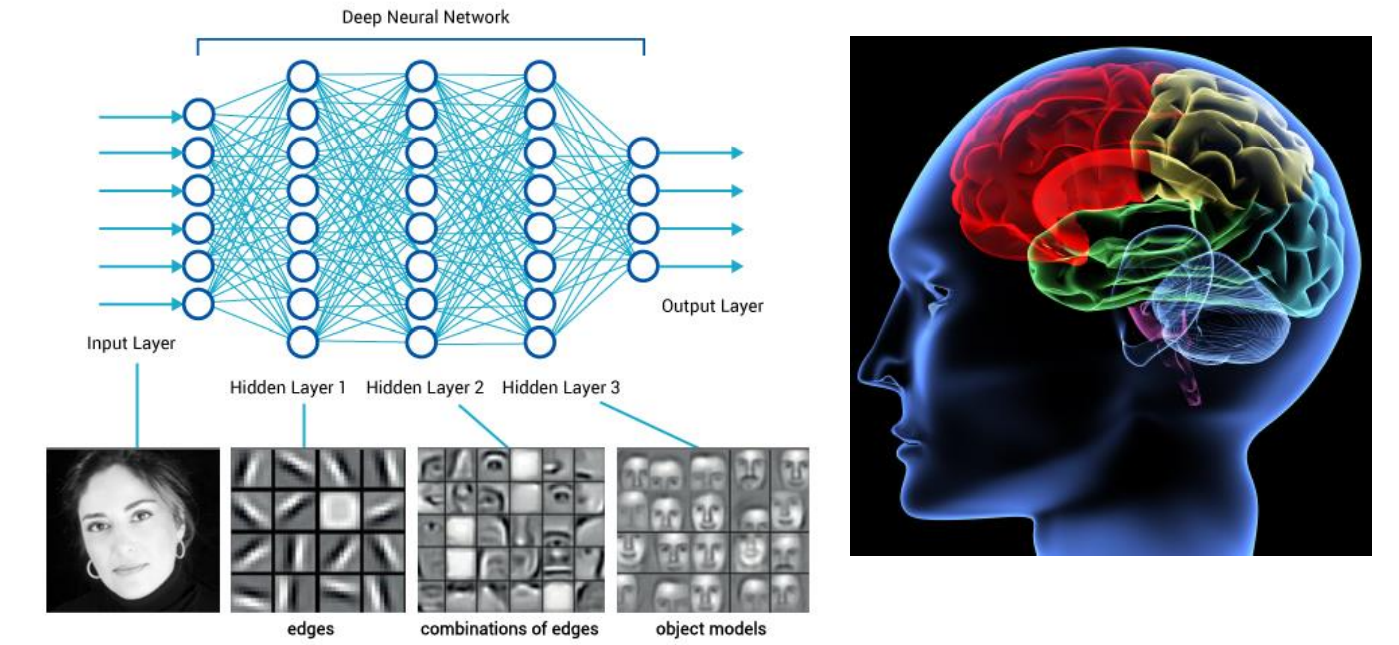
\includegraphics[scale=0.45]{deeplearning.png}
\caption{Mô tả mô hình một mạng neuron học sâu}
\end{figure}

\paragraph{Lịch sử xu hướng của học sâu:}
\begin{itemize}
\item Học sâu xuất hiện từ xưa nhưng đã dẫn không còn phổ biến do nhiều lí do.
\item Học sâu đã trở lại  và trở nên rất hữu khi có rất nhiều dữ liệu để huấn luyện.
\item Mô hình học sâu phát triển nhanh chóng theo thời gian khi cơ sở hạ tâng cho học sâu ngày càng được cải thiện. 
\item Các vấn đề học sâu giải quyết được có độ phức tạp ngày càng tăng đi đôi với độ chính xác cũng vậy.
\end{itemize}
\section{Các thành phần quan trọng trong mô hình học sâu}
Neuron là đơn vị nhỏ nhất của mạng neuron, chúng có cấu tạo như sau: 
\begin{figure}[H]
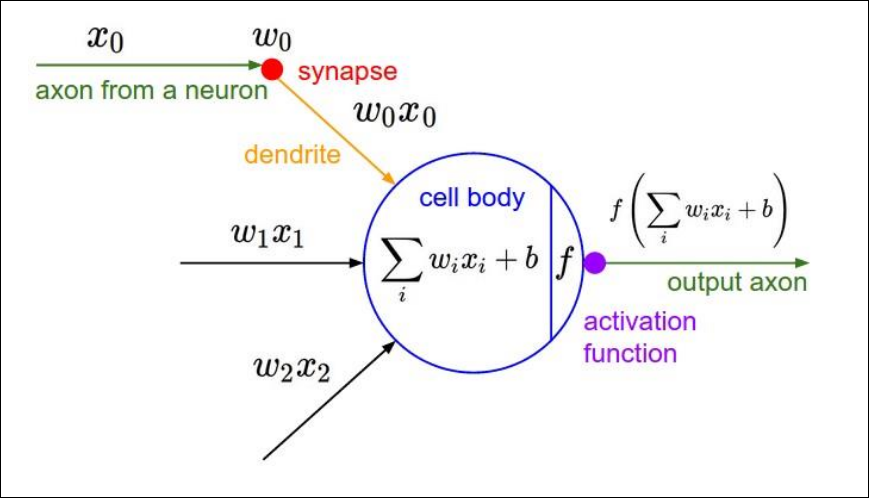
\includegraphics[scale=0.45]{aneuron.png}
\caption{Cấu trúc của một neuron}

\end{figure}
\begin{itemize}
\item Các tín hiệu đầu vào $x_0,x_1,...$
\item Đầu vào tổng thể là tích hợp của các tín hiệu đầu vào $ \sum_i w_ix_i+b$ với  $w_i$ là trong số gán với đầu vào $x_i$

\item Hàm mục tiêu:\\ Các hàm mục tiêu hay được sử dụng \begin{itemize}
\item sigmoid $\sigma =1/(1+e^-x)$
\item tanh $ tanh(x)$
\item ReLU $ max(0,x)$
\item ELU \abovedisplayskip=0pt\relax
\begin{equation}
\begin{cases}
x \qquad \qquad \qquad  if x>0\\ \alpha (exp(x)-1) \quad if x \leq 0
\end{cases}
\end{equation}
\item Maxout $max(w_1^T x+b_1,w_2^T x+b_2) $

\end{itemize}
\end{itemize}


\paragraph{Kiến trúc mạng} 
\begin{figure}[H]
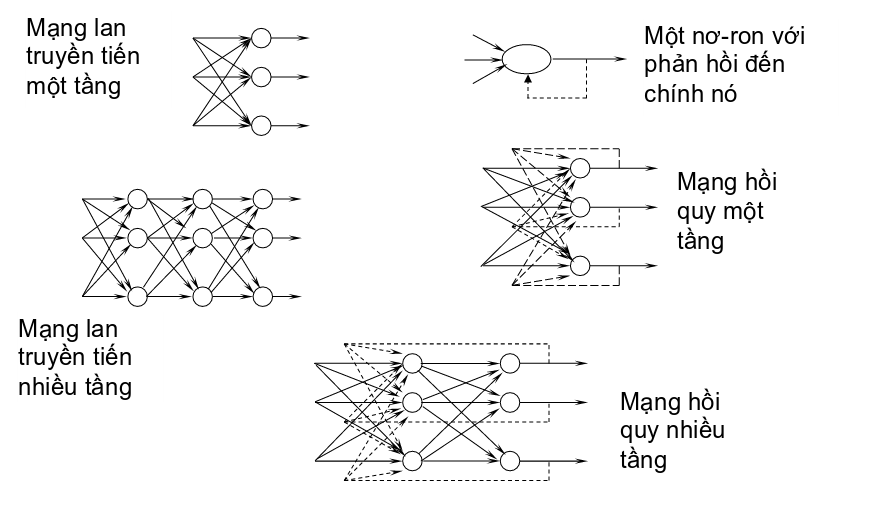
\includegraphics[scale=0.45]{archneuron.png}
\caption{Các kiến trúc mạng neuron điển hình}
\end{figure}
\begin{itemize}
\item Một mạng neuron lân truyền tiến nếu không có bất kì đầu ra của nút nào là đầu vào của một neron cùng tầng.
\item Khi đầu ra của một nút là đầu vào của nút ở cùng tẩng hoặc tầng trước thì đó là mạng phản hồi.
\item Nếu tạo thành một chu trình thì đó là mạng hồi quy.
\end{itemize}
\paragraph{Thuật toán học:} Với một mạng neuron lan truyền tiến, hiện tại thuật toán lan truyền ngược vẫn là thuật toán được sử dụng rộng rãi và đem lại hiệu quả cao.
\paragraph{Chiến lược học:} Với những bài toán phức tạp chiến lược học Gradient Descent tỏ ra rất chậm và hiệu quả không cao dưới đây là nhưng chiến lược học khác có tốc độ nhanh và đem lại hiệu quả không kém hơn Gradient Descent thông thường:
\begin{itemize}
\item Stochastic Gradient Descent
\item Mini-batch Gradient Descent
\item SGD-Momentum
\item SGD-Vanilla
\item Adagrad
\item AdaDelta
\end{itemize}

\chapter{Giới thiệu mạng CNN}\label{chap_CNN}
\section{Kiến trúc tổng quan của CNN}\label{sec_intro_cnn}
Giống như mạng neuron thông thường đã được giới thiệu phần trước, CNN nhận đầu vào và biến đổi đầu vào đó thông qua một loạt các tầng ẩn. Mỗi tầng ẩn được tạo thành từ một tập các neuron, trong đó nếu như mạng neuron thông thường mỗi một neuron trong mỗi tầng ẩn được kết nối đầy đủ với các neuron thuộc tầng liền trước đó thì mỗi neuron trong tầng ẩn của mạng CNN sẽ không kết nối với toàn bộ các neuron thuộc tầng liền trước (đây chính là điểm khác biệt lớn nhất của CNN so với mạng neuron thông thường).
\begin{figure}[H]
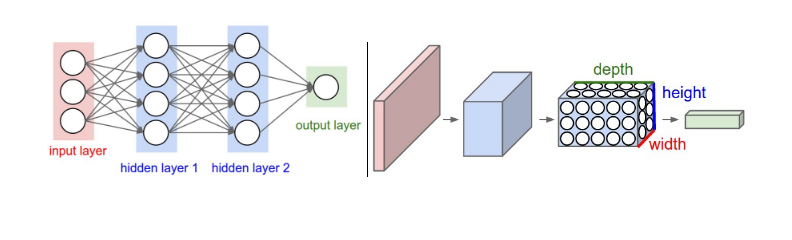
\includegraphics[scale=0.7]{img1.png}
\caption{Mô hình tổng quan ANN vs CNN}
\end{figure}
Trong bài toán phân loại ảnh, mỗi tầng của CNN sẽ nhận đầu vào là một khối 3 chiều (width, height, depth) xử lý và đưa ra đầu ra cũng là khối 3 chiều và phụ thuộc vào các tham số của mỗi tầng mà kích thước đầu ra có thể biến đổi theo từng chiều. Trong kiến trúc CNN gồm 3 tầng chính đó là: Convolution Layer, Pooling Layer, Fully-connected Layer.

\section{Convolution Layer (CONV)}\label{sec_intro_conv}
Convolution Layer là tầng cốt lõi của mạng CNN \\ 

\textbf{Tổng quan:} Tham số của lớp CONV bao gồm một tập hợp các bộ lọc. Mỗi bộ lọc là một không gian nhỏ chiều rộng và chiều cao là các tham số cần chọn và kéo dài qua toàn bộ chiều sâu của khối đầu vào. Mỗi một bộ lọc sẽ trượt trên toàn chiều rộng và chiều cao của khối đầu vào và tính toán các sản xuất nhân giữa các ô của bộ lọc và các đầu vào tại vị trí tương ứng mà bộ lọc trượt qua. \\ 

\textbf{Quan điểm não:}  Mỗi mục trong khối lượng đầu ra 3D cũng có thể được hiểu như là một sản phẩm của một tế bào thần kinh mà nhìn vào chỉ một vùng nhỏ trong các tham số đầu vào. \\ 
 
\textbf{Kết nối địa phương:} Khi làm việc với các đầu vào nhiều chiều như hình ảnh, sẽ không phù hợp nếu mỗi neuron ở tầng phía sau sẽ kết nối đầy đủ với toàn bộ các neuron thuộc tầng phía trước. Thay vào đó, chúng ta sẽ kết nối mỗi neuron ở tầng phía sau với một khu vực địa phương của khối đầu vào. Phạm vi không gian của kết nối này là một siêu tham số gọi là khu vực tiếp nhận (bằng với kích cỡ của bô lọc) và kết nối dọc theo trục chiều sâu của khối đầu vào.
\begin{figure}[H]
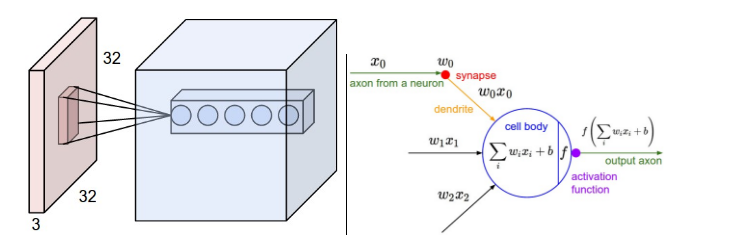
\includegraphics[scale=0.7]{img2.png}
\caption{CONV Layer}
\end{figure}
\textbf{Sắp xếp không gian:} Không gian số lượng các neurons ở đầu ra của mỗi khối làm thế nào để sắp xếp chúng. Ở đây có 3 siêu tham số dùng để kiểm soát kích thước của khối lượng đầu ra:depth(độ sâu), stride(sải chân) vào đệm (zero-padding):
\begin{itemize}
\item[1. ] Thứ nhất, độ sâu của khối lượng đầu ra là một hyperparameter: nó tương ứng với số lượng bộ lọc chúng tôi muốn sử dụng, mỗi học tập để tìm kiếm một cái gì đó khác nhau trong các đầu vào.
\item[2. ] Thứ hai, chúng ta phải xác định các stride mà chúng ta trượt lọc. Khi stride là 1 sau đó chúng tôi di chuyển các bộ lọc một điểm ảnh tại một thời điểm. Khi stride là 2 (hoặc khác thường 3 hoặc nhiều hơn, mặc dù điều này là hiếm trong thực tế) sau đó các bộ lọc nhảy 2 điểm ảnh tại một thời điểm khi chúng ta đẩy chúng xung quanh. Điều này sẽ tạo ra khối lượng sản lượng nhỏ không gian.
\item[3. ] Thứ ba, đôi khi để thuân tiện hơn để lề bao quanh ngoài của ảnh với số không. Các kích thước này zero-padding là một hyperparameter. Điểm hay của zero-padding là nó sẽ cho phép chúng ta kiểm soát kích thước không gian của khối lượng đầu ra (thường gặp nhất như chúng ta sẽ thấy sớm, chúng ta sẽ sử dụng nó để bảo toàn chính xác kích thước không gian của khối lượng đầu vào để các đầu vào và đầu ra rộng và chiều cao đều giống nhau).
\end{itemize} 

\textbf{Tham số không gian:} Nó chỉ ra rằng chúng ta có thể làm giảm đáng kể số lượng các thông số bằng cách làm cho một giả định hợp lý: đó, nếu một tính năng rất hữu ích để tính toán tại một số vị trí không gian (x, y), sau đó nó nên cũng có ích để tính toán tại một vị trí khác nhau (x2 , y2). Nói cách khác, biểu thị một lát 2 chiều duy nhất của chiều sâu như một lát độ sâu. Trong thực tế trong quá trình lan truyền ngược, mỗi tế bào thần kinh trong khối lượng sẽ tính toán gradient cho trọng lượng của nó, nhưng các gradients sẽ được thêm lên trên mỗi miếng chiều sâu và chỉ cập nhật một bộ trọng lượng mỗi slice. \\
 
\textbf{Tóm lại:}Lớp Conv Layer
\begin{itemize}
\item Đầu vào một khối lượng kích thước $W_1*H_1*D_1$.
\item Yêu cầu 4 siêu tham số:
\begin{itemize}
\item Số bộ lọc K,
\item Kích cỡ mỗi bộ lọc F,
\item Bước sải S,
\item Số lương của lề (zeros-padding) P
\end{itemize}
\item Tạo ra 1 khối có kích cỡ $W_2*H_2*D_2$
\begin{itemize}
\item $W_2= \frac{(W_2 - F + 2P)}{S} + 1$
\item $H_2=\frac{(H_1 - F + 2P)}{S}+1$(chiều cao và chiều rộng tính như nhau bởi đối xứng).
\item $D_2 = K$.
\item Với chia sẻ tham số,$F*F*D_1$ trọng số/mỗi bộ lọc. Tổng trọng số là $(F*F*D_1)*K$ và K là biases.
\item Trong khối lượng đầu ra,độ sâu lát thứ d(kích cỡ $W_2*H_2$) là kết quả của việc thực hiện một chập hợp lệ của bộ lọc thứ d với đầu vào có sải là S,và sau đó bù lại bởi bias thứ d.
\end{itemize}
\end{itemize}
Một cài đặt thông thường các siêu tham só là $F = 3, S = 1, P= 1 $. Tuy nhiên, có những quy ước chung và quy tắc vận dụng mà thúc đẩy các siêu tham
\begin{center}
\begin{figure}[H]
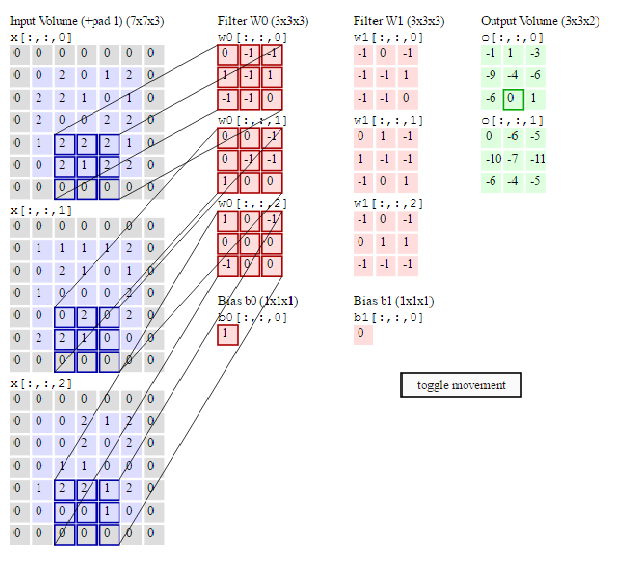
\includegraphics[scale=0.7]{img3.png}
\caption{Ví dụ CONV}
\end{figure}
\end{center}
\section{Pooling Layer}
Nó được phổ biến định kỳ thêm một layer Pooling ở giữa lớp Conv liên tiếp trong một kiến trúc ConvNet. Chức năng của nó là để dần dần làm giảm kích thước không gian của các đại diện để giảm số lượng các thông số và tính toán trong mạng, và vì thế để kiểm soát cũng overfitting. Các Pooling lớp hoạt động độc lập trên mỗi lát chiều sâu của đầu vào và thay đổi kích thước nó về không gian, sử dụng các hoạt động MAX. Các hình thức phổ biến nhất là một lớp tổng hợp với các bộ lọc kích thước $2*2$ áp dụng với một sải chân của 2 downsamples mỗi lát sâu trong đầu vào của 2 dọc theo cả hai chiều rộng và chiều cao,loại bỏ $75\%$ các kích hoạt.Mỗi hoạt động MAX sẽ trong trường hợp này là dùng một tối đa hơn 4 số (vùng $2*2$ ít trong một số lát chiều sâu). Chiều sâu vẫn không thay đổi. Tổng quát hơn, các lớp tổng hợp:
\begin{itemize}
\item Đầu vào là các khối kích thước $W_1*H_1*D_1$.
\item Yêu cầu 2 tham số
\begin{itemize}
\item Phạm vi không gian(F)
\item Các bước tiến(S)
\end{itemize}
\item Sản xuất một khối lượng kích thước $W_2*H_2*D_2$ ở đây:
\begin{itemize}
\item $W_2 =\frac{(W_1 - F)}{S} + 1$
\item $H_2 =\frac{(H_1 - F)}{S} + 1$
\item $D_2 = D_1$
\end{itemize}
\item Tham số zeros-padding khi nó tính một hàm cố định của các đầu vào
\item Lưu ý rằng nó không phải là phổ biến để sử dụng zero-đệm cho việc kết hợp các lớp
\end{itemize}
\begin{center}
\begin{figure}[H]
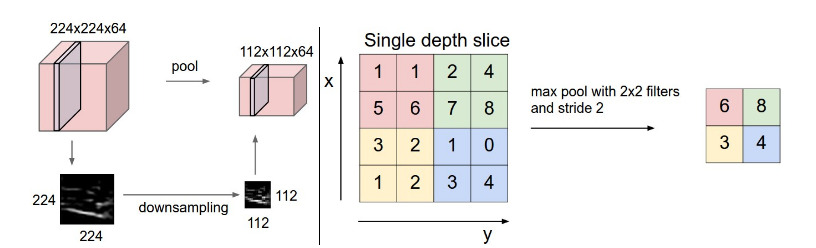
\includegraphics[scale=0.8]{img4.png}
\caption{Ví dụ CONV}
\end{figure}
\end{center}
\section{Fully-connected Layer(kết nối đầy đủ)}
Tế bào thần kinh trong một lớp đầy đủ kết nối có các kết nối đầy đủ với tất cả các kích hoạt trong lớp trước, như đã thấy trong thường xuyên Neural Networks. Kích hoạt của họ do đó có thể được tính toán với một phép nhân ma trận theo sau là một xu hướng bù đắp. Xem các Neural Network phần của các ghi chú để biết thêm thông tin.
\section{Các lớp mẫu của mô hình về CNN}
Các hình thức phổ biến nhất của một kiến trúc ConvNet xếp một vài lớp CONV-RELU, sau đó với lớp POOL, và lặp đi lặp lại mô hình này cho đến khi hình ảnh đã được sáp nhập về không gian đến một kích thước nhỏ. Tại một số điểm, nó được phổ biến để chuyển đổi sang lớp kết nối đầy đủ. Các lớp kết nối đầy đủ cuối cùng nắm giữ đầu ra, chẳng hạn như điểm số lớp. Nói cách khác, kiến trúc ConvNet phổ biến nhất theo mẫu sau: \\
\\
\small{
\textbf{INPUT -> [[CONV -> RELU]*N -> POOL?]*M -> [FC -> RELU]*K -> FC}
}
\\ \\
Ở đây * chỉ ra sự lặp lại, và POOL? chỉ ra một lớp tổng hợp tùy chọn. Hơn nữa, N >= 0(và thường N <= 3), M >= 0, K >= 0(và thường K < 3)


\chapter{Google Inception}
\section{Inception Module \cite{googlenet}}	
Mục đích chính của các kiến mạng neuron là trích rút các đặc trưng của dữ liệu đầu vào. Thông thường, dữ liệu đầu vào thường có cấu trúc thưa (ví dụ đầu vào là ảnh cần trích rút các điểm ảnh đặc trưng của ảnh đầu vào trong số nhiều điểm ảnh nhiễu (điểm ảnh không phải là trọng tâm của ảnh)). Nếu như trong kiến trúc của mạng CNN, mỗi tầng convolution chỉ có một tập các filter có kích thước cố định trượt trên không gian đầu vào thì ý tưởng trong kiến trúc inception là để trích rút hết các đặc trưng của đầu vào thay vì nhìn dữ liệu theo 1 cách ở mỗi tầng (sử dụng các filter có kích thước giống nhau) thì sẽ nhìn dữ liệu theo nhiều cách (sử dụng các filter có kích thước khác nhau để trượt qua không gian đầu vào). Để đảm bảo việc sử dụng các filter có kích thước khác nhau tại mỗi tầng mà vẫn đảm bảo độ phức tạp tính toán của mạng, kiến trúc inception đã sử dụng kỹ thuật giảm chiều dữ liệu trước khi tính toán với filter lớn (chi phí tính toán cao). Các filter ở mỗi tầng sẽ được gộp lại và được gọi là inception module.

\subsection{Inception module naive version}
Trong phiên bản này, chỉ cân nhắc đến việc nhìn dữ liệu theo nhiều cách khác nhau bằng cách sử dụng các filter có kích thước khác nhau tại cùng một tầng mà chưa tính đến việc giảm chiều dữ liệu trước khi tính toán phức tạp. 
\begin{figure}[H]
\centering
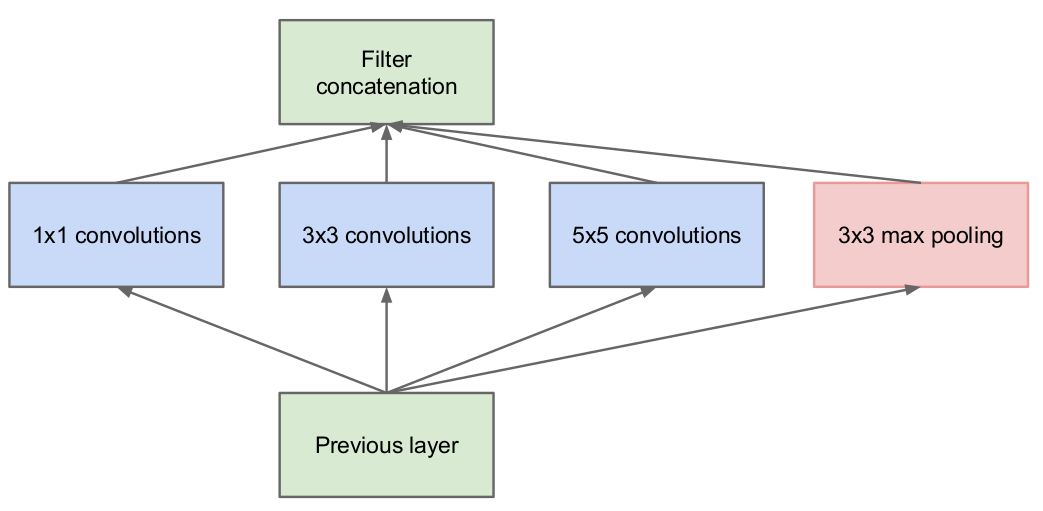
\includegraphics[scale=0.45]{inception_naive.png}
\caption{Inception module naive version}
\end{figure}
Trong đó \textbf{Filter concatenation} để gộp các output của các tầng convolution.Ví dụ: Output của các tầng $1 \times 1$, $3 \times 3$, $5 \times 5$ convolution lần lượt là $H \times W \times C_1$, $H \times W \times C_3$, $H \times W \times C_5$ thì output của inception module là $H \times W \times (C_1+C_3+C_5)$
\subsection{Inception module với kỹ thuật giảm chiều}
Để giảm chi phí tính toán, trước khi tính toán với các filter lớn ($3\times 3$ và $5 \times 5$) thì sử dụng các filter kích thước $1 \times 1$ để giảm chiều dữ liệu sẽ giúp cho giảm chi phí tính toán (số lượng tham số, khối lượng tính toán) (Ví dụ: Hình \ref{fig_reduce1x1})
\begin{figure}[H]
\centering
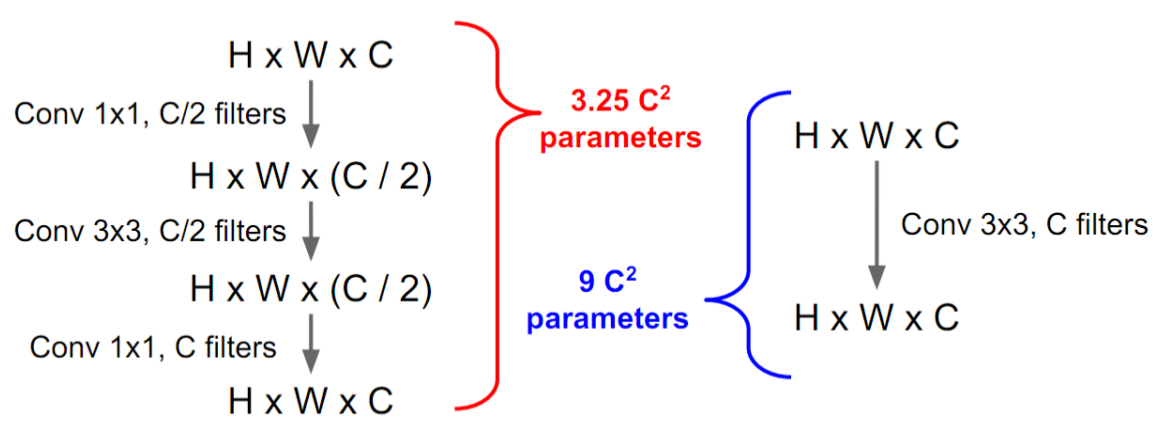
\includegraphics[scale=0.4]{reduce_1x1.png}
\caption{Giảm chiều dữ liệu với filter $1 \times 1$}
\label{fig_reduce1x1}
\end{figure}
\par Dựa vào tính chất đó, trong Inception module naive version, trước khi tính áp dụng các filter $3 \times 3$, $5 \times 5$ lên input, ta sẽ giảm chiều input qua các filter $1 \times 1$ (Hình \ref{fig_inception_reduce})
\begin{figure}[H]
\centering 
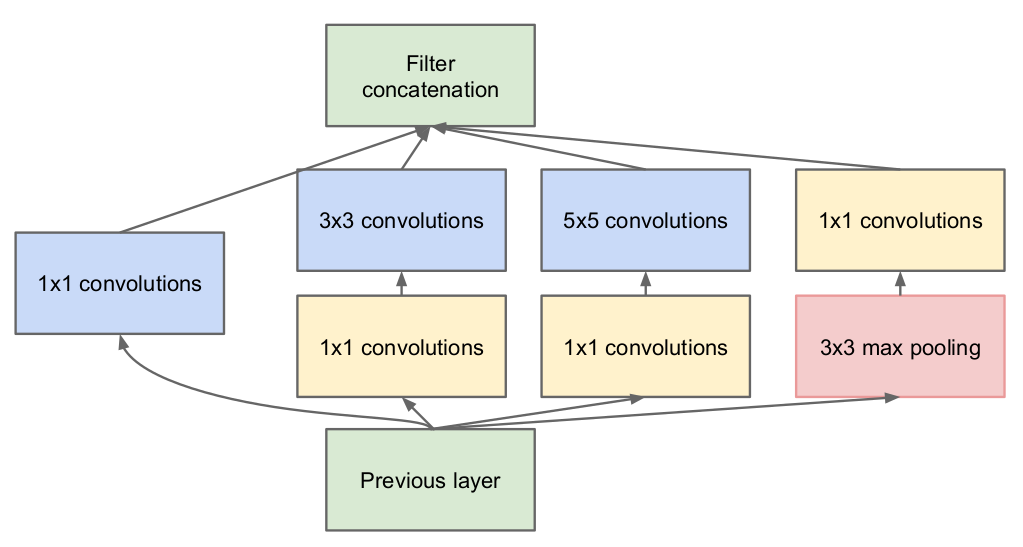
\includegraphics[scale=0.45]{inception_reduce.png}
\caption{Inception module với kỹ thuật giảm chiều}
\label{fig_inception_reduce}
\end{figure}

\subsection{GoogLeNet}
GoogLeNet là tên mạng sử dụng kiến trúc inception trong cuộc thi ILSVRC 2014. GoogLeNet sử dụng kiến trúc inception với Inception module với kỹ thuật giảm chiều. Cụ thể kiến trúc mạng của GoogLeNet được mô tả trong hình \ref{fig_googLeNet}
\begin{figure}[H]
\centering 
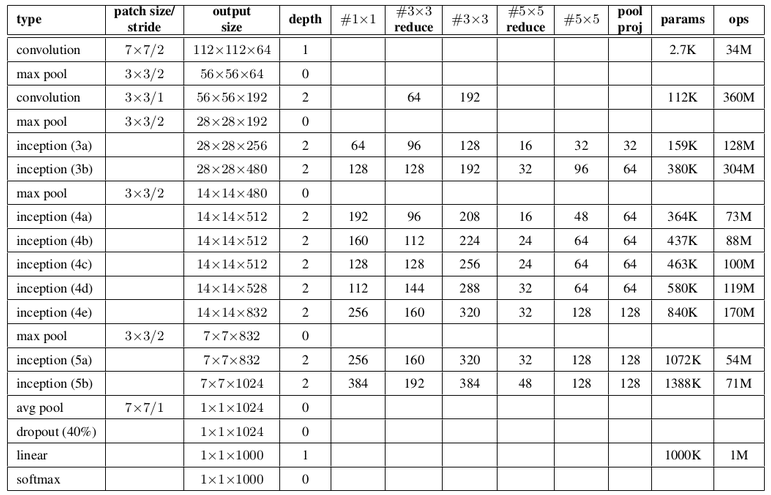
\includegraphics[scale=0.65]{googLeNet.png}
\caption{Kiến trúc GoogLeNet}
\label{fig_googLeNet}
\end{figure}

\section{Inception v4 \cite{rethinking} \cite{inceptionv4}}
\subsection{Cải tiến Inception module}
\par Giả sử ta đặt 2 tầng Convolution (với kích thước filter mỗi tầng là $3 \times 3$ và stride là 1) cạnh nhau (stack) thì mỗi neuron thuộc tầng convolution thứ 2 sẽ nhìn vào một vùng kích thước $5 \times 5$ trong khối đầu vào của tầng thứ convolution thứ nhất (Hình \ref{fig_2conv3x3}). 
\begin{figure}[H]
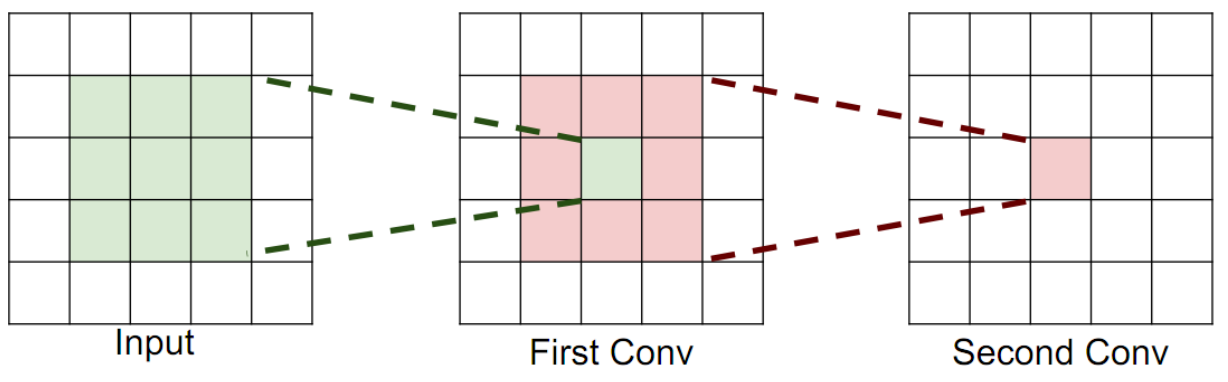
\includegraphics[scale=0.5]{2conv3x3.png}
\caption{stack 2 tầng $3 \times 3$ convolution}
\label{fig_2conv3x3}
\end{figure}
\par Thay vì stack 2 tầng convolution, nếu stack 3 tầng convolution (với kích thước filter mỗi tầng là $3 \times 3$ và stride là 1) thì mỗi neuron ở tầng convolution cuối cùng sẽ nhìn một vùng có kích thước $7 \times 7$ của khối đầu vào của tầng convolution đầu tiên (Hình \ref{fig_3conv3x3})
\begin{figure}[H]
\centering
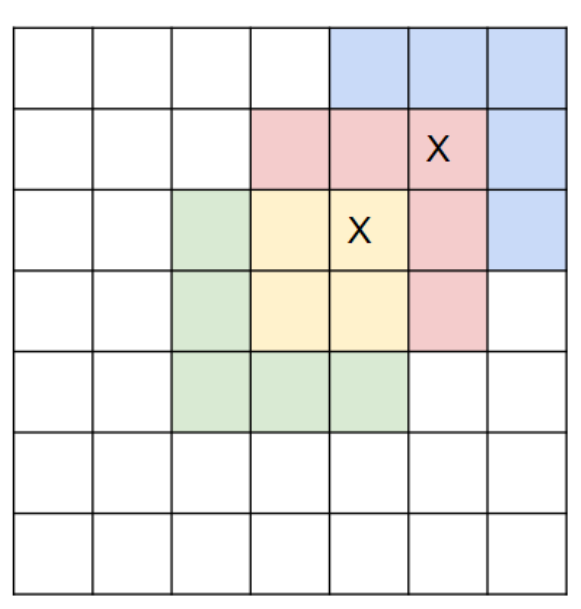
\includegraphics[scale=0.4]{3conv3x3.png}
\caption{stack 3 tầng $3 \times 3$ convolution}
\label{fig_3conv3x3}
\end{figure}
\par Giả sử có một khối đầu vào có kích thước $H \times W \times C$ nếu đi vào một tầng convolution có $C$ filter kích thước $7 \times 7$ (với stride = 1 và padding để bảo toàn kích thước đầu vào) thì số lượng tham số sẽ là: $C \times (7 \times 7 \times C) = 49C^2$ và khối lượng tính toán (số lượng phép toán) là: $(H \times W \times C) \times (7 \times 7 \times C) = 49HWC^2$ còn nếu cũng với khối kích thước đầu vào đó nếu đi vào stack 3 tầng convolution cũng có $C$ filter (với stride = 1 và padding để bảo toàn kích thước đầu vào) nhưng với kích thước $3 \times 3$ ở mỗi tầng thì số lượng tham số sẽ là : $3 \times C \times (3 \times 3 \times C) = 27C^2$ và khối lượng tính toán là: $3 \times (H \times W \times C) \times (3 \times 3 \times C) = 27HWC^2$
\par Qua ví dụ trên có thể thấy, thay vì sử dụng một tầng convolution với kích thước filter của tầng đó là lớn (ví dụ $7 \times 7$) thì việc stack nhiều tầng convultion có kích thước nhỏ hơn (ví dụ $3 \times 3$) sẽ giúp giảm số lượng các tham số và khối lượng tính toán của mạng. Thêm vào đó việc sử dụng nhiều tầng convolution sẽ giúp cho tính phi tuyến của hàm mà mạng học được tăng lên. Áp dụng nhận xét đó ta có cải tiến của inception module (Hình \ref{fig_inception_reduce}) bằng cách thay một tầng convoluiton với filter có kích thước $5 \times 5$ bằng 2 tầng convolution với filter ở mỗi tầng có kích thước $3 \times 3$ (Hình \ref{fig_replace_5x5vs3x3})
\begin{figure}[H]
\centering 
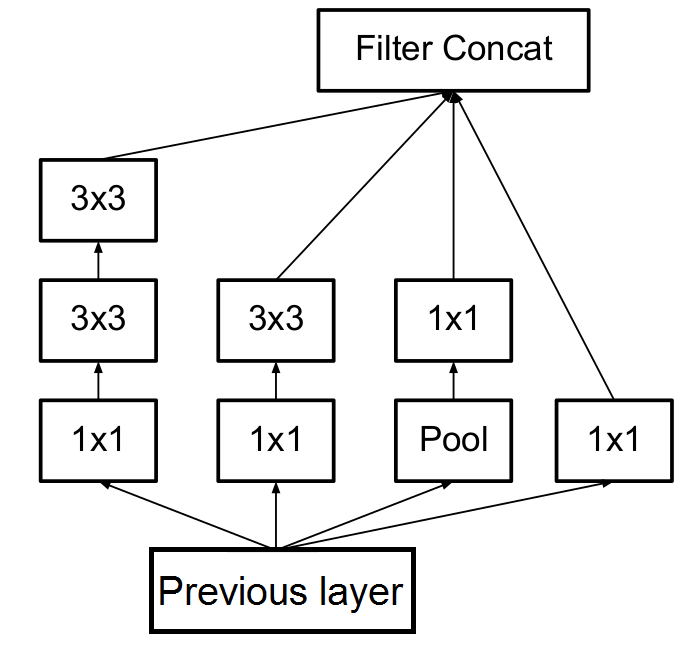
\includegraphics[scale=0.4]{replace_5x5vs3x3.png}
\caption{Inception module khi thay 1 convolution $5 \times 5$ bằng 2 convolution $3 \times 3$}
\label{fig_replace_5x5vs3x3}
\end{figure}
\par Như đã trình bày ở phần trên, việc thay một tầng convoluiton với filter có kích thước $5 \times 5$ bằng 2 tầng convolution với filter ở mỗi tầng có kích thước $3 \times 3$ sẽ giúp giảm tham số, giảm chi phí tính toán. Vậy tại sao không thay 1 tầng convolution với filter có kích thước $3 \times 3$ bằng 2 tầng convolution với filter ở mỗi tầng có kích thước $2 \times 2$.
\par Cũng với ví dụ ở phần trên, giả sử có một khối đầu vào có kích thước $H \times W \times C$ nếu đi vào 2 tầng convolution có $C$ filter kích thước $2 \times 2$ (với stride = 1 và padding để bảo toàn kích thước đầu vào) thì số lượng tham số sẽ là: $2 \times C \times (2 \times 2 \times C) = 8C^2$ và khối lượng tính toán (số lượng phép toán) là: $2 \times (H \times W \times C) \times (2 \times 2 \times C) = 8HWC^2$. Nếu cũng với khối đầu vào đó đi vào 1 tầng convolution có $C$ filter kích thước $1 \times 3 $ sau đó đi vào 1 tầng convolution có $C$ filter kích thước $3 \times 1$ (cả 2 tầng đều cso tham số stride = 1 và padding để bảo toàn kích thước đầu vào)thì số lượng tham số là: $C \times 1 \times 3 \times C+ C \times 3 \times 1 \times C = $ và khối lượng tính toán là: $(H \times W \times C) \times (1 \times 3 \times C) + (H \times W \times C) \times (3 \times 1 \times C) = 6HWC^2$

\par Như vậy, qua ví dụ trên ta có thể thấy, việc thay một tầng convolution có kích thước filter $3 \times 3$ bằng 2 tầng convolution có kích thước fiter ở mỗi tầng lần lượt là $1 \times 3$ và $3 \times 1$ sẽ tiết kiệm được số lượng tham số và khối lượng tính toán hơn việc thay một tầng convolution có kích thước filter $3 \times 3$ bằng 2 tầng convolution có kích thước fiter ở mỗi tầng là $2 \times 2$ (33\% của 2 filter $1 \times 3$ và $3 \times 1$ so với 11\% của 2 filter $2 \times 2$). Sau khi tách mỗi tầng convolution có kích thước filter $3 \times 3$ bằng 2 tầng convolution có kích thước fiter ở mỗi tầng lần lượt là $1 \times 3$ và $3 \times 1$ ta thu được inception module như hình \ref{fig_fac_3x3}
\begin{figure}[H]
\centering 
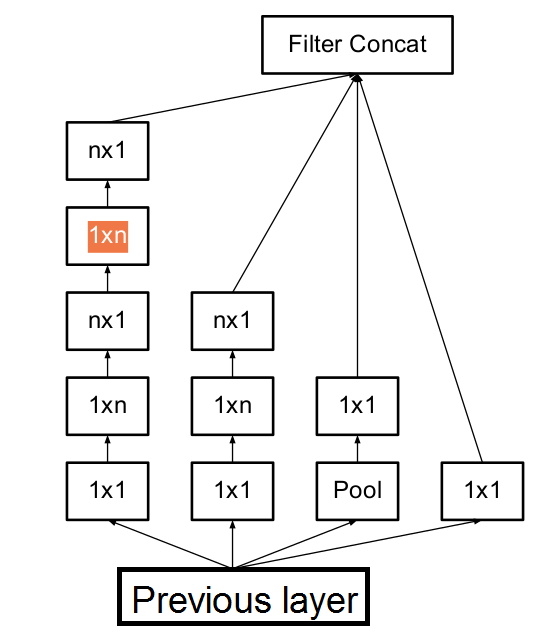
\includegraphics[scale=0.5]{fac_3x3.png}
\caption{Inception module sau khi phân rã $3 \times 3$ convolution (n = 3)}
\label{fig_fac_3x3}
\end{figure}

\subsection{Inception v4}
Mạng inception v4 tích hợp inception module và các cải tiến của nó (Hình \ref{fig_inceptionv4}).
\begin{figure}[H]
\centering 
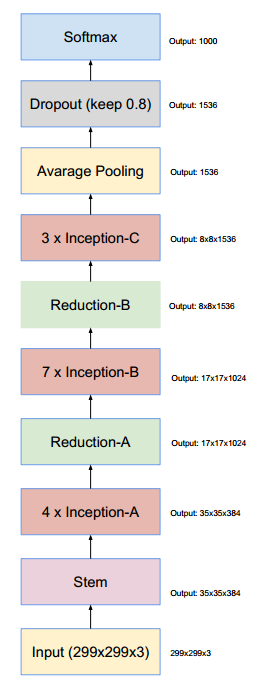
\includegraphics[scale=0.7]{inceptionv4.png}
\caption{Kiến trúc mạng inception v4}
\label{fig_inceptionv4}
\end{figure}
\par Inception-A là inception module sau khi thay 1 tầng convolution với filter $5\times 5$ bằng 2 tầng convolution với kích thước filter của mỗi tầng là $3 \times 3$ (Hình \ref{fig_inceptionA})
\begin{figure}[H]
\centering 
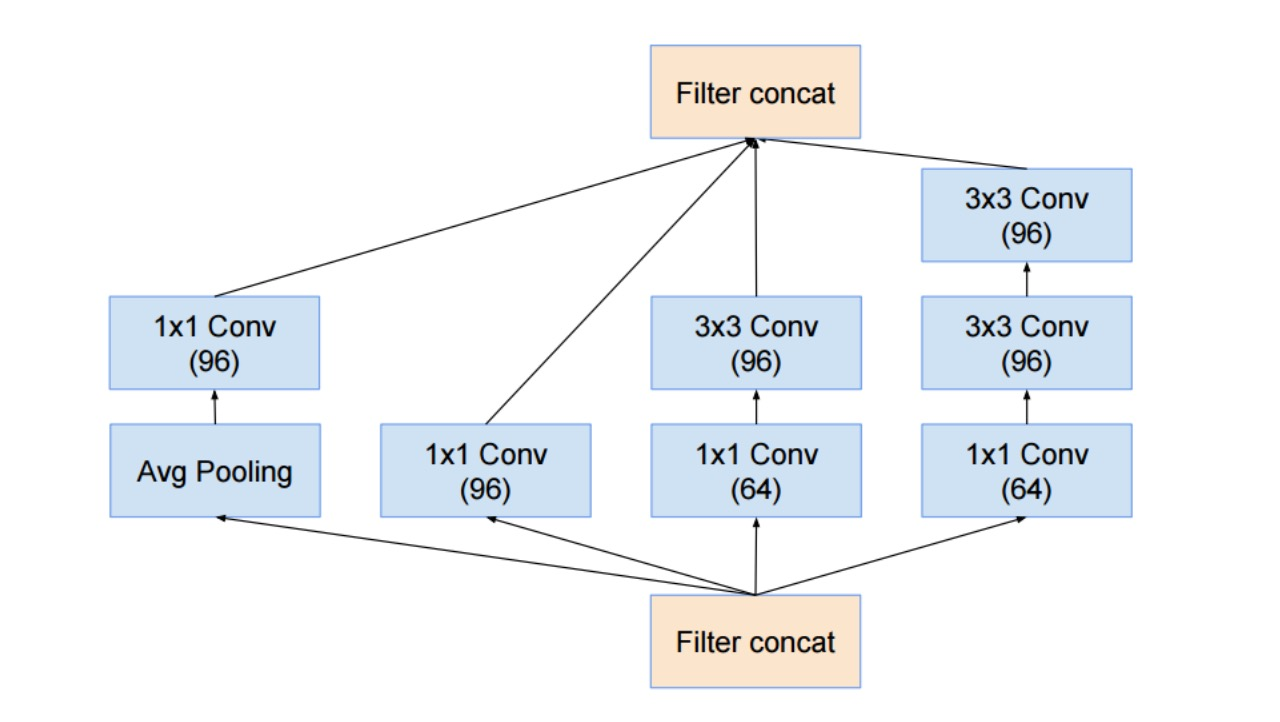
\includegraphics[scale=0.4]{inceptionA.jpg}
\caption{Inception-A}
\label{fig_inceptionA }
\end{figure}
\par Inception-B áp dụng kỹ thuật phân rã tầng convolution $n \times n$ thành các convolution $1 \times n$ và $n \times 1$ (với n = 7) (Hình \ref{fig_inceptionB})
\begin{figure}[H]
\centering 
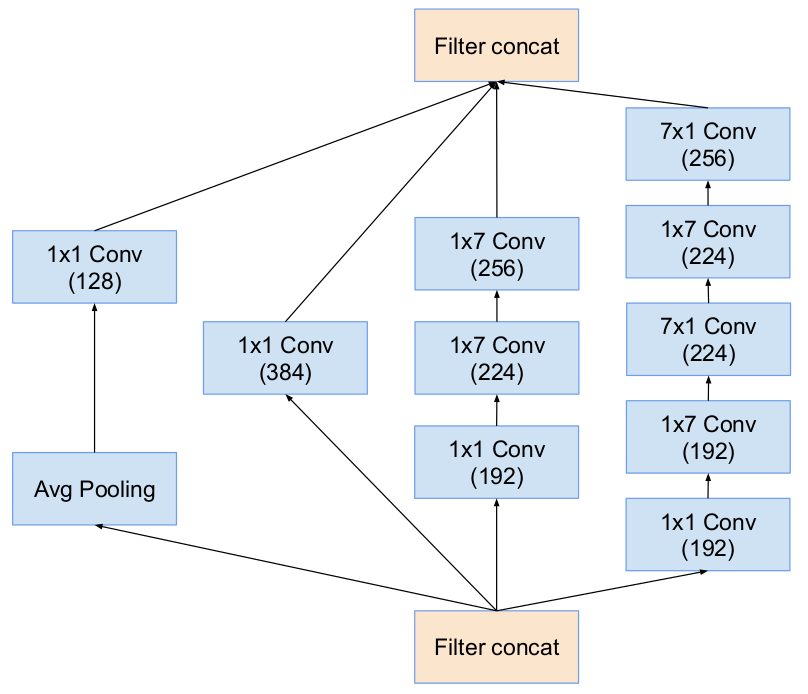
\includegraphics[scale=0.5]{inceptionB.png}
\caption{Inception-B}
\label{fig_inceptionB}
\end{figure}


\begin{thebibliography}{9}
\bibitem{googlenet} C. Szegedy, W. Liu, Y. Jia, P. Sermanet, S. Reed, D. Anguelov, D. Erhan, V. Vanhoucke, and A. Rabinovich. \textit{Going deeper with convolutions}

\bibitem{rethinking} C. Szegedy, V. Vanhoucke, S. Ioffe, J. Shlens, and Z. Wojna. \textit{Rethinking the inception architecture for computer vision}

\bibitem{inceptionv4} C. Szegedy, S. Ioffe, and V. Vanhoucke. \textit{Inception-v4, Inception-ResNet and the Impact of Residual Connections on Learning}

\bibitem{slidesangdv} Slide DeepLearning, Thầy Đinh Viết Sang 

\end{thebibliography}

\end{document}
